\documentclass{szzclass}

\usepackage{amsmath}
\usepackage{graphics}
\usepackage[export]{adjustbox}[2011/08/13]
% \usepackage[czech]{babel}
% \usepackage[margin=3cm]{geometry}
% \usepackage{wrapfig}

% % spacing
% \usepackage{titlesec}
% % \titlespacing*{\section}{0pt}{1ex}{0.5ex}
% \titlespacing*{\subsection}{0pt}{1ex}{0ex}

\topic{Procesy a vlákna, jejich implementace. Synchronizační nástroje.
Klasické synchronizační úlohy. Plánování vláken. Přidělování prostředků,
Coffmanovy podmínky, způsoby řešení uváznutí.}
\renewcommand*\contentsname{Obsah}
\author{Daniel Hampl}
\code{BI-SPOL-16}
\subject{OSY}

\begin{document}
% \maketitle

\tableofcontents
\newpage


\section{Procesy a vlákna}

\textbf{Program}
je posloupnost instrukcí definujících chování procesu.

\textbf{Proces}
je instance spuštěného programu, která
slouží k alokování prostředků (adresový prostor, otevřené soubory, ... ).
Informace o tomto procesu (ID, identita, informace o rodiči a potomcích,...) jsou následně uloženy v jádru.

\textbf{Vlákno}
je část výpočtu, které je přidělován procesor (jádro CPU).
Jádro alokuje pro každé vlákno zásobník (pro historii výpočtu a lokální proměnné) a udržuje aktuální hodnoty registrů (pro opětovné spuštění)

\subsection{Procesy}
\textbf{Vytvoření}
\begin{itemize}
    \item OS inicializuje v jádře datové struktury spojené s novým procesem.
    \item OS nahraje kód a data programu z disku do paměti a vytvoří prázdný systémový zásobník pro main vlákno.
\end{itemize}

\textbf{Klonovaní}
\begin{itemize}
    \item OS zastaví aktuální proces a uloží jeho stav.
    \item OS inicializuje v jádře datové struktury spojené s novým procesem.
    \item OS udělá kopii aktuálního kódu, dat, zásobníku, stavu procesu,...
\end{itemize}

\textbf{fork()}
\begin{itemize}
    \item Vytvoří nový proces, který je kopií procesu, z kterého byla tato funkce zavolána.
    \item V rodičovském procesu vrací funkce PID potomka
    \item V potomkovi vrací funkce 0
    \item Kódový segment sdílí potomek s rodičem.
    \item Datový a zásobníkový segment vznikají kopií dat a zásobníku rodiče.
\end{itemize}

\textbf{execve(char *filename,...)}
\begin{itemize}
    \item V procesu, ze kterého je funkce volána, spustí nový program.
    \item Obsah původního procesu je přepsán novým programem.
    \item Atributy procesu se nemění (PID, PPID, ...).
\end{itemize}

\textbf{wait(int *status)}
\begin{itemize}
    \item Umožňuje v rodičovském procesu počkat na dokončení potomka.
    \item Funkce zablokuje rodičovský proces, ve kterém je zavolána, dokud se jeden potomek neukončí.
\end{itemize}

\textbf{Ukončení}
\begin{itemize}
    \item Proces se pokusí předat návratový kód rodiči
    \item Ukončení všech vláken, která existují v rámci procesu
    \item Uvolnění aresového prostoru procesu a jeho datových struktu
\end{itemize}

\subsection{Vlákna}

\begin{itemize}
    \item Jsou jednotky plánované pro spuštění na CPU
    \item Každé vlákno má vlastní:
    \begin{itemize}
        \item Hodnotu čítače instrukcí
        \item Hodnotu CPU registrů
        \item Zásobník
    \end{itemize}
    \item Ostatní prostředky jsou sdílené
    \item Vlákna nejsou nezávislá jako procesy
    \item Vlákna sdílí stejný adresový prostor, stejné soubory, potomky a reakce na signály
\end{itemize}

\begin{figure}[h]
    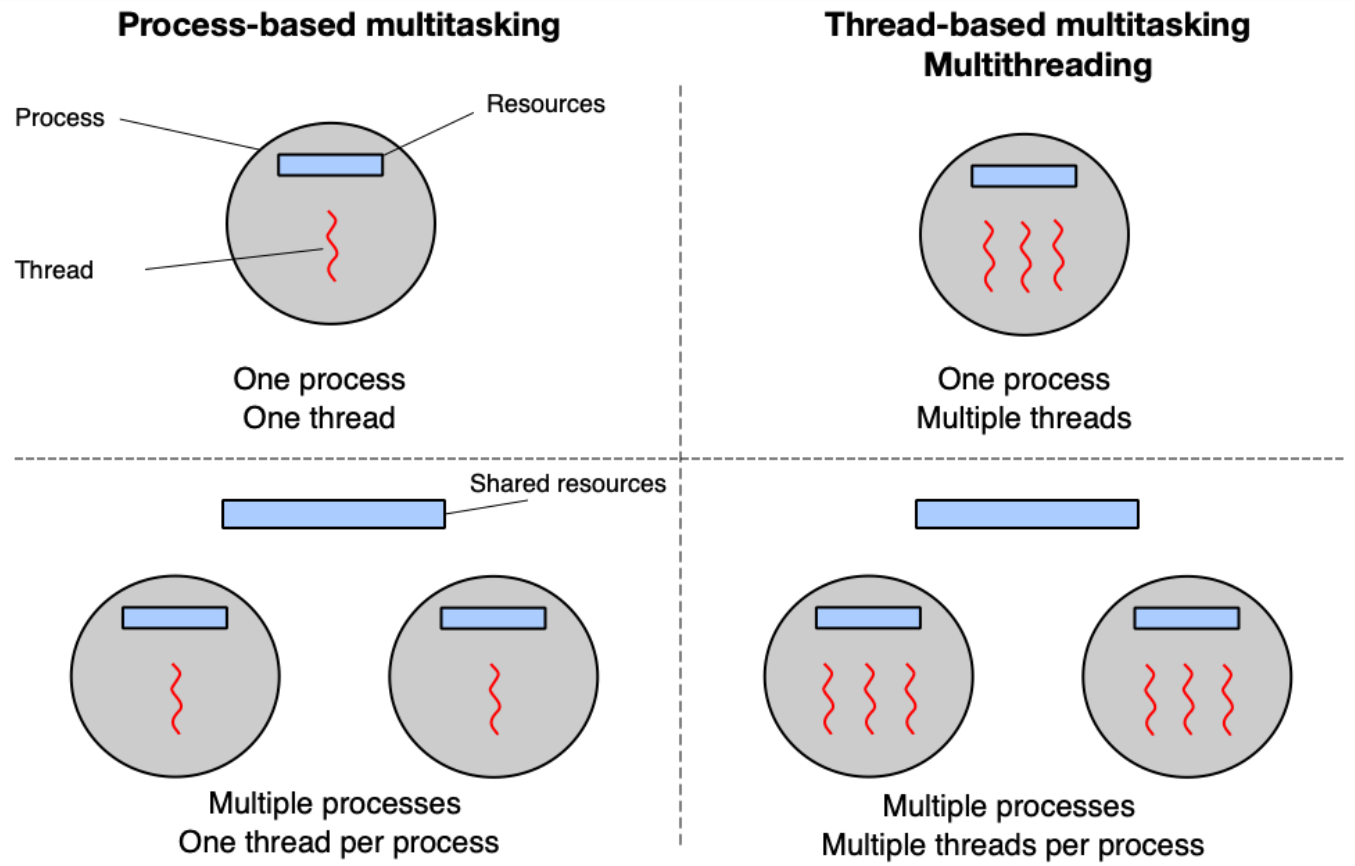
\includegraphics[width=.8\textwidth, center]{topics/bi-spol-16/images/multitask.png}
\end{figure}

\textbf{Vytvoření}
\begin{itemize}
    \item pthread\_create() v POSIXu
    \item CreateThread() v MS Win
\end{itemize}

\textbf{Ukončení}
\begin{itemize}
    \item pthread\_exit() POSIX
    \item ExitThread() MS Win
\end{itemize}

\newpage

\textbf{Přepínání kontextu}
\begin{itemize}
    \item Rozdělení vláken jednotlivých procesů mezi jednotlivá jádra
    \item Vlákno má svojí dobu, po kterou může běžet na daném jádře, pak je prerušeno a je dán čas jinému vláknu
\end{itemize}

\begin{figure}[h]
    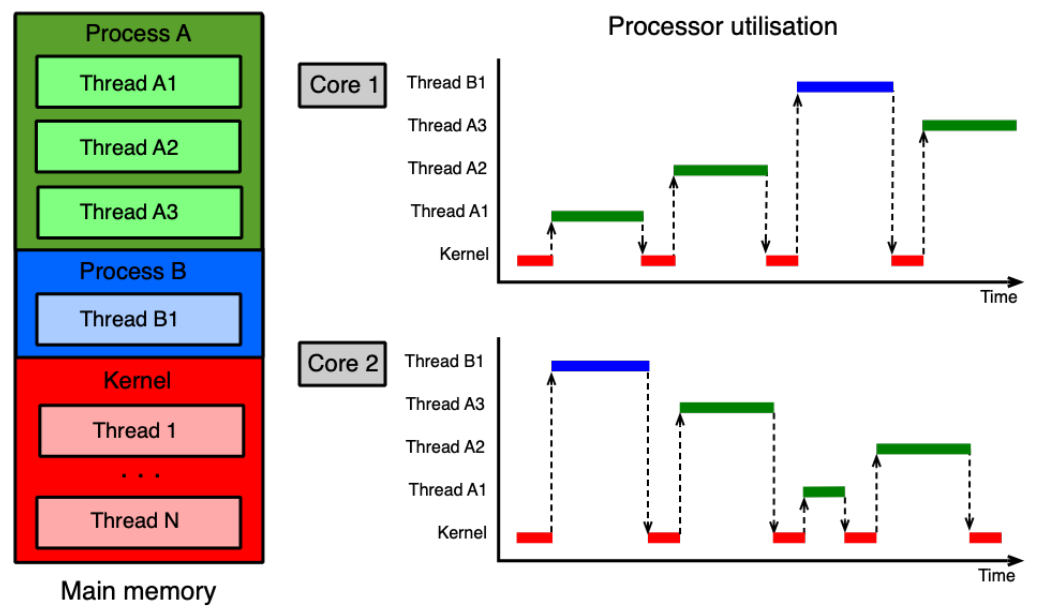
\includegraphics[width=.8\textwidth, center]{topics/bi-spol-16/images/thread1.png}
\end{figure}


\textbf{Stavy vláken}
\begin{itemize}
    \item Idle: vznik nového vlákna
    \item Ready: vlákno čeká až mu bude přiďeleno jádro CPU
    \item Running: vlákno je zpracováváno jádrem CPU
    \item Blocked: vlákno čeká na událost (dokončení I/O operace, příchod signálu,...)
    \item Zombie: vlákno je ukončováno, ale zatím ještě nebylo vše dokončeno
    \item Free: vlákno bylo kompletne zrušeno (pouze teoretický stav)
\end{itemize}

\begin{figure}[h]
    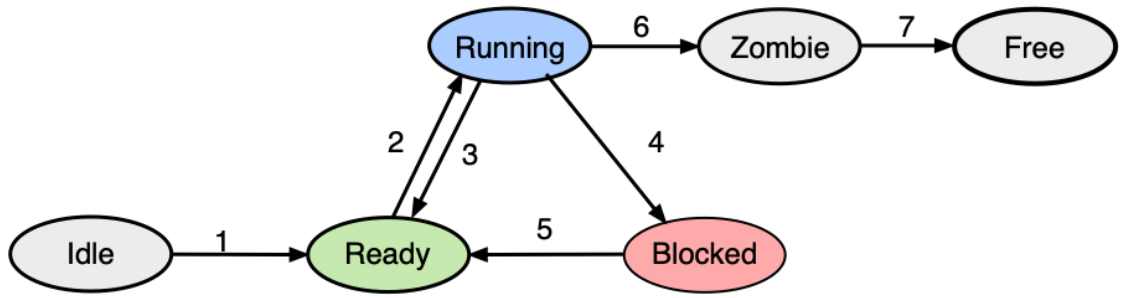
\includegraphics[width=.8\textwidth, center]{topics/bi-spol-16/images/stavy.png}
\end{figure}

\newpage

\section{Synchronizace}

\subsection{Zákaz přerušení (DI)}

CPU je přidělováno postupně jednotlivým vláknům za pomoci přerušení od časovače nebo jiného přerušení.
Vlákno zakáže všechna přerušení před vstupem do kritické sekce a opět je povolí až po jejím opuštění.

\subsubsection{Nevýhody}
\begin{itemize}
    \item DI od jednoho uživatele blokuje i ostatní
    \item V multi-CPU má efekt pouze na aktuální CPU
    \item Zpomalí reakce na přerušení
    \item Možnost blokovat celé CPU při chybné implementaci
    \item Nehodí se pro běžná uživatelská vlákna
\end{itemize}

\subsection{Aktivní čekání vs blokování}

Pouze jedno vlákno může do kritické sekce, ostatní mají smůlu

\subsubsection{Aktivní čekání}

\begin{itemize}
\item Sdílená proměnná indikuje obsazenost
\item Vlákna ve smyčce testují tuto hodnotu a čekají až budou moci postoupit
\item Pokud se dlouho čeká na vstup do kritické sekce, dochází k plýtvání časem procesoru
\end{itemize}

\subsubsection{Blokování}

Vlákno provede systémové volání, které ho zablokuje do okamžiku než se sekce uvolní

\subsection{Sdílená proměnná}

Vzájemné vyloučení nastavením sdílené proměnné při vstupu do sekce

\subsection{Instrukce TSL}
\begin{itemize}
    \item Test and Set Lock (TSL) - instrukce načte obsah slova do registru a nastaví obsah slova na nenulovou hodnotu
    \item CPU provádějící TSL lockne paměťovou sběrnici dokud se TSL nedokončí
    \item TSL je atomická instrukce
    \item TSL lze použít u multi-cpu se sdílenou pamětí
\end{itemize}


\subsection{Instrukce XCHG}
\begin{itemize}
    \item Alternativa k TSL
    \item Exchange instrukce (XCHG) atomicky prohodí obsah slova na dané adrese v paměti a registru
\end{itemize}

\subsection{Problémy}

\subsubsection{Bez použití synchronizace (časově závislé chyby)}
\begin{itemize}
    \item Dva a více procesů či vláken používá společné prostředky (sdílená paměť, soubor, proměnná)
    \item Výsledek je závislý na přepínání kontextu
    \item Tyto chyby jsou velmi špatně detekovatelné
\end{itemize}


\subsubsection{Při použití synchronizace}
\begin{itemize}
    \item Deadlock = situace kdy se více vláken čeká na událost, kterou může vyvolat pouze jedno z čekajících vláken
    \item Livelock = situace, kdy několik vláken vykonává neužitečnou činnost (mění svůj stav), ale nemohou postoupit k vykonávání usefull práce
    \item Hladovění = situace, kdy ready vlákno je předbíháno a nedostane se k prostředkům
\end{itemize}

\subsubsection{Inverzní prioritní problém}

\begin{itemize}
\item Vlákno A má nižší prio. a je v kritické sekci
\item Vlákno B má vyšší prio. a čeká pomocí aktivního čekání
\item OS používá prioritní plánování, má 1 jádro na 1 CPU
\item Potom může nastat, je-li priorita fixní, uváznutí
\end{itemize}

\subsubsection{Synchronizace pomocí blokování}
\begin{itemize}
\item Ve většina případů je blokování lepší než aktivní čekání či zákaz přerušení
\item Vlákno je zablokováno, pokud chce vstoupit do již zablokované kritické sekce, je přesunuto na čekací frontu
\item Tyto operace již na úrovni jádra OS
\end{itemize}

\subsection{Typy synchronizace}

\begin{itemize}
\item Blokující send i receive - rendevous
\item Neblokující send a blokující receive
\item Neblokující send i receive + test příchozích zpráv
\end{itemize}

\subsection{Adresování}

\begin{itemize}
\item Přímé - Zpráva je uložena přímo do prostoru příjemce
\item Nepřímé - Zpráva je uložena do sdíleného prostoru (mailbox)
\end{itemize}

\section{Přidělování prostředků}

\subsection{Sleep \& Wakeup}

\subsubsection{wait()}

\begin{itemize}
\item Systémové volání
\item Zablokuje vlákno, které ho zavolalo
\item Zakáže alokaci CPU pro toto vlákno a přesune jej do fronty, kde čeká na probuzení
\end{itemize}

\subsubsection{wakeup(thread)}

\begin{itemize}
\item Probudí vlákno uspané pomocí wait()
\item Odstraní vlákno z čekací fronty
\item Povolí alokaci CPU
\item Waiting bit
\begin{itemize}
    \item Wakeup volání na neuspané vlákno - bit je nastaven
    \item Uspání vlákna s již nastaveným bitem - vlákno není uspáno, ale bit je pouze resetován
\end{itemize}
\end{itemize}


\subsection{Condition variable}

\subsubsection{cond\_wait(\&var, \&mutex)}

\begin{itemize}
\item Mutex zamčen a daném vláknu
\item Po zavolání je mutex odemčen a vlákno uspáno
\item Po probuzení je mutex znovu uzamčen
\end{itemize}

\subsubsection{cond\_signal(\&var)}

Odblokuje alespoň jedno z uspaných vláken

\newpage

\subsection{Semafor}

\begin{itemize}
    \item Obsahuje čítač a frontu čekajících procesů
    \item Instrukce jsou prováděny atomicky (nelze je přerušit)
    \item \textbf{Init()}\newline
    Nastavení čítače na zadané číslo a vyprázdní se fronta
    \item \textbf{Down()}\newline
    Pokud je čítač > 0, sníží se o jedna. V opačném případě je vlákno uloženo do fronty.
    \item \textbf{Up()}\newline
    Pokud je fronta neprázdná, probudí se jedno z čekajících vláken. V opačném případě se navýší čítač o jedna.
    \item \textbf{Monitory}\newline
    Do bloku je vpuštěno vždy jen jedno vlákno\newline
    O vyloučení v rámci bloku se stará překladač nikoli programátor
    \item \textbf{wait(c)}\newline
    Pozastaví vlákno na podmíněné proměnné c
    \item \textbf{signal(c)}\newline
    Probudí jedno z pozastavených vláken
\end{itemize}

\subsection{Bariéry}
Propouští minimální počet vláken. Když vlákna přijdou k bariéře, tak čekají, dokud jich není minimální počet, a až poté jsou puštěny dál



\section{Coffmanovy podmínky}
\begin{itemize}
    \item Uváznutí nastane pouze pokud jsou splněny následující podmínky.
\begin{enumerate}
    \item \textbf{Vzájemné vyloučení:}
    každý prostředek je buď přidělen právě jednomu vláknu
    a nebo je volný (prostředek nemůže být sdílen více vlákny).
    \item \textbf{Podmínka neodnímatelnosti:} prostředek, který byl již
    přidělen nějakému vláknu, nemůže mu být násilím odebrán
    (musí být dobrovolně uvolněn daným vláknem).
    \item \textbf{Podmínka "drž a čekej":} vlákno, které má již přideleny
    nějaké prostředky, může žádat o další prostředky
    (vlákno může žádat o prostředky postupně).
    \item \textbf{Podmínka kruhového čekání:} musí existovat smyčka
    dvou nebo více vláken, ve které každé vlákno čeká na prostředek
    přidelený dalšímu vláknu ve smyčce.
\end{enumerate}
\item První tři podmínky jsou nutné ale ne dostačující $\implies$ k
uváznutí může dojít. Poslední podmínka představuje samotné uváznutí.
\item Pokud aspon jedna z podmínek není splněna, nemůže dojít k uváznutí.
\end{itemize}
\section{Uváznutí}
\subsection{Způsoby řešení uváznut}

\subsubsection{Pštrosí algoritmus}
Úplné ignorování celého problému. 

\subsubsection{Detekce a zotavení}
K uváznutí může dojít, ale pak je detekováno a odstraněno

Zotavení pomocí odebrání - násilné odebrání prostředku

Zotavení pomocí návratu - při detekci uváznutí je proces vrácen zpět v čase

Zotavení pomocí ukončení procesů - ukončení procesu ze smyčky alokačního grafu

\subsubsection{Pečlivá alokace prostředků}

\subsubsection{Prevence pomocí nesplnění aspoň jedné z Coffmanových podmínek}

\section{Příklady}

\subsection{Večeřící filosofové}
Model vláken, které soutěží o výlučný přístup k omezenému počtu prostředků.

N filozofů sedí kolem kulatého stolu a každý z nich buď přemýšlí nebo jí. K jídlu potřebuje současně levou a pravou vidličku.

Řešení:
\begin{itemize}
    \item Pomocí mutexu
    \item Ověřovani že můžeme vzít obě vidličky (atomické)
    \item Upozornění sousedů po skončení
    \item Sousedi blokováni mutexem než dostanou upozornění
\end{itemize}



\subsection{Čtenáři - písaři}
Model vláken, které přistupují do společné databáze.

Více čtenářů může číst současně data pokud žádný písař nemodifikuje data v databázi.

Pouze jeden písař může modifikovat data v databázi v jednom okamžiku.

Řešení:
\begin{itemize}
    \item Pomoc mutexu a counteru
    \item Uzavírání DB při psaní
    \item Reader čeká než může číst
    \item Reader notifikuje writer když už nikdo nečte
    \item Writer čeká než může psát
    \item Writer notifikuje reader když už nepiše
\end{itemize}

\subsection{Producent - konzument}
\textbf{Producent} produkuje data a vkládá je do sdílené fronty s omezenou kapacitou

\textbf{Konzument} vybírá data ze sdílené fronty.

Řešení:
\begin{itemize}
    \item Tři mutexy
    \item Jeden pro prřístup do fronty
    \item Jeden pro stav full (konzument čeká)
    \item Jeden pro stav empty (producent čeká)
\end{itemize}




\end{document}
